\section{Théorie}
\begin{wrapfigure}{R}{0.5\linewidth}
    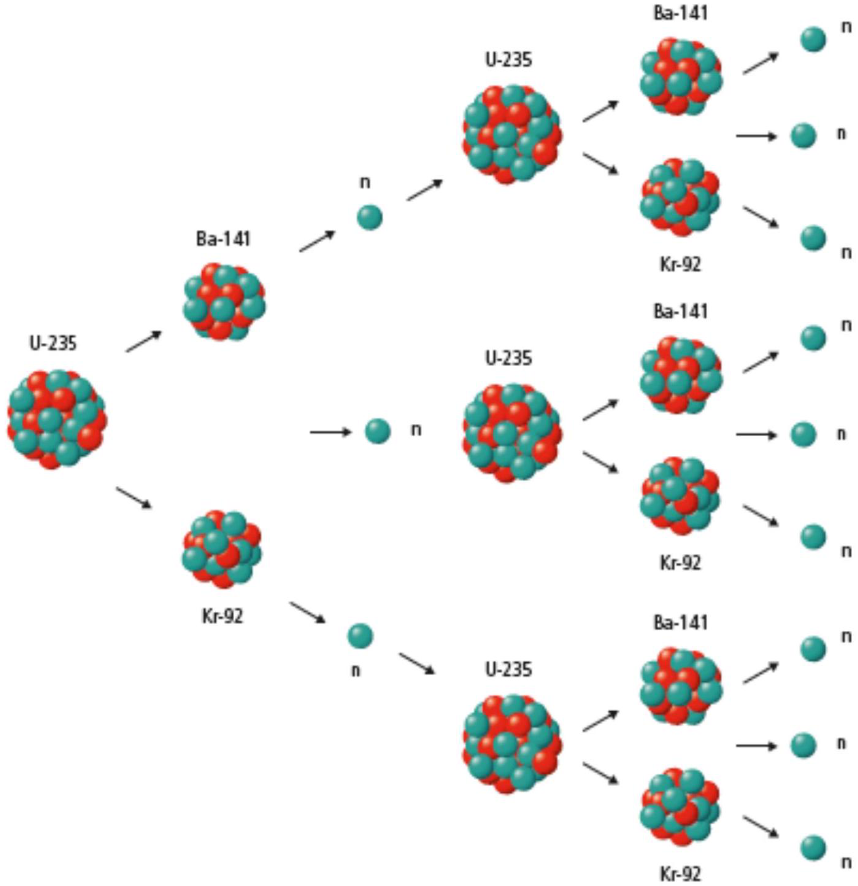
\includegraphics[width=\linewidth]{figures/fission.png}
    \caption{Schéma d'une réaction en chaîne de fission nucléaire avec de l'uranium 235 \cite{notice}}
    \label{fig:fission}
\end{wrapfigure}
Les réacteurs de fission nucléaire produisent de l'électricité en utilisant l'énergie provenant de la fission des atomes afin de chauffer de l'eau pour faire tourner une turbine. La fission des atomes lourds tels que l'uranium 235 ($\mathrm{U}^{235}$) libère en effet de grandes quantités d'énergie par rapport à des réactions chimiques, telles que la combustion pour les énergies fossiles, car elle revient à briser les liens dans les noyaux des atomes. La chaleur libérée $\mathrm{Q}$ est ainsi de l'ordre de \mbox{200 \si{\mega\electronvolt}} pour la fission d'un atome d'uranium 235 \cite{notice}. Cette densité énergétique représente un des principaux intérêts de l'énergie nucléaire et de l'uranium 235 comme combustible. Celui-ci n'est cependant présent dans la nature qu'à hauteur de 0.72\% de l'uranium total et il est nécessaire d'enrichir l'uranium naturel pour des applications énergétiques \cite{notice}.

Il s'agit donc d'étudier plus précisément la fission de l'uranium 235 et le comportement général d'un réacteur à fission nucléaire. Le noyau de l'uranium 235 se scinde lorsqu'il est percuté par un neutron $n$ selon l'équation de fission:
\begin{equation}
    n + \mathrm{U}^{235} \to 2\cdot \mathrm{PF} + \bar{v} \cdot n + \mathrm{Q}
    \label{eq:fission-u235}
\end{equation}
où PF représente des produits de fission de numéros atomiques plus bas que l'uranium et $\bar{v}$ le nombre moyen de neutrons produits par la fission (pour l'$\mathrm{U}^{235}$, $\bar{v} \approx 2.5$). Les neutrons produits par la fission vont ensuite théoriquement provoquer d'autres réactions de fission dans le combustible et ainsi poursuivre une réaction en chaîne comme illustré en \autoref{fig:fission}. Cependant les neutrons libérés dans l'\autoref{eq:fission-u235} possèdent une énergie d'environ 2 \si{\mega\electronvolt}, trop élevée pour avoir une forte probabilité de provoquer une nouvelle fission. Ils doivent donc être ralentis à l'aide d'un modérateur à noyaux légers. Pour les réacteurs à eau légère (LWR) cela correspond à l'eau. Le niveau d'eau $h$ dans le réacteur détermine donc la proportion de neutrons qui pourront déclencher de nouvelles fissions. Pour caractériser cela le facteur de multiplication effectif est défini comme:
\begin{equation}
    k_\mathrm{eff} = \frac{\mathrm{Production \, de \, neutrons}}{\mathrm{Absorptions} + \mathrm{Fuites}}
\end{equation}
La condition de criticité correspondant à une puissance constante provenant d'un nombre de fissions constant et elle obtenue avec:
\begin{equation}
    \mathrm{Production \, de \, neutrons} = \mathrm{Absorptions} + \mathrm{Fuites} \Rightarrow k_\mathrm{eff} = 1
\end{equation}
sont également définis les conditions sous-critique, $k_\mathrm{eff} < 1$, et sur-critique, $k_\mathrm{eff}>1$, qui correspondent respectivement à une diminution et une augmentation exponentielles du nombre de fissions par seconde et donc de la puissance du réacteur.

Pour étudier ces conditions de criticité, des détecteurs de neutrons sont placés proches du coeur du réacteur et donnent soit un courant d'intensité $I$ soit un compte du nombre de neutrons. En relevant le nombre de neutrons $N$ lors d'un intervalle de temps $t$ il est possible d'obtenir le compte de neutrons par seconde $C$. Ces deux détecteurs sont tels que $I$ et $C$ sont proportionnels au flux de neutron $\Phi$ lui même dépendant d'une source de neutrons $S$ et du facteur $k_\mathrm{eff}$. Ainsi:
\begin{equation}
    \begin{aligned}
        & \Phi \propto \frac{S}{1 - k_\mathrm{eff}} \\
        & \Rightarrow \frac{1}{I} \, , \frac{1}{C} \propto \frac{1}{\Phi} \propto (1 - k_\mathrm{eff})
    \end{aligned}
    \label{eq:proportionalities}
\end{equation}
$k_\mathrm{eff}$ étant lui même dépendant de la hauteur d'eau $h$ il est possible d'approximer une relation linéaire entre $1/I$ ou $1/C$ et $h$. De cette manière à la hauteur d'eau critique $h_C$, $k_\mathrm{eff}=1$ et donc selon ces relations $1/I = 0$ et $1/C = 0$. Il est en pratique impossible d'obtenir $I = \infty$ et $C = \infty$ mais cela permet d'extrapoler une valeur de $h_C$.

Lors de l'étude d'un réacteur nucléaire il est important d'attendre la stabilisation du compte de neutrons car les réactions de fission produisent également de plusieurs manières des atomes radioactifs. Ceux-ci peuvent se désintégrer en produisant eux même d'autres neutrons, dits retardés, n'apparaissant pas immédiatement après le changement du niveau du modérateur.